\documentclass[11pt]{article}

\usepackage[margin=1in]{geometry}
\usepackage{graphicx}
\usepackage{amsmath}
\usepackage{float}
\usepackage{setspace}
\usepackage{hyperref}
\usepackage{longtable}

\setlength{\parskip}{0.5em}
\setlength{\parindent}{0em}
\onehalfspacing

\title{BlueAlpha1 Interim Report (Winter 2026)\\
Prior Sensitivity Analysis Framework for Bayesian Marketing Mix Models}
\author{
Aidan Frazier \and Quinlan Wilson \and Jimmy Wu \and Jasper Luo \and Coraline Zhu
}
\date{March 20, 2026}

\begin{document}
\maketitle

\section{Introduction}
Marketing Mix Models (MMM) help organizations estimate how marketing channels contribute to business outcomes and support budget decisions. In our project, we use a Bayesian MMM workflow built on Google Meridian \cite{meridian_model_spec,meridian_configure}. A practical advantage of Bayesian MMM is that analysts can encode prior beliefs about channel performance. A practical risk is that posterior ROI estimates may become sensitive to those priors, especially when signal strength is weak or channels are correlated, a pattern emphasized in prior Bayesian MMM literature \cite{jin2017}.

Our project objective is to build a reproducible sensitivity framework that stress-tests ROI conclusions under different prior assumptions before those conclusions are used for decision-making. This report summarizes progress through Winter 2026, with emphasis on the linked-target experiment for \texttt{google, meta, tiktok}. The rest of the report is organized as follows: Section 2 states the problems of interest, Section 3 describes materials and methods, Section 4 presents preliminary findings, Section 5 discusses interpretation and challenges, and Section 6 outlines future work.

\section{Problems of Interest}
We focus on two high-level problems that align with our capstone objectives.

Problem 1: \textbf{Robustness of channel ROI conclusions under prior changes.} We want to know whether core ROI conclusions are stable when prior mean, prior scale, and prior family are varied over plausible ranges.

Problem 2: \textbf{Practical risk translation.} We want sensitivity outputs that can be interpreted in business terms (not only percent changes), so teams can identify which channels carry the highest decision risk when priors are misspecified.

\section{Materials and Methods}
\subsection*{Data and Modeling Context}
Input data comes from \texttt{data/raw/monthly\_mocha.csv}. The outcome variable is subscriptions, and channel-level media variables include impressions and spend columns. The modeled channel set is:
\texttt{meta, google, snapchat, tiktok, moloco, liveintent, beehiiv, amazon}.

The Winter interim analysis reported here uses linked-target perturbation for \texttt{google, meta, tiktok}, while still estimating ROI for all modeled channels in each run.

\subsection*{Prior-Sensitivity Design}
We use a prior grid over three components:
\begin{itemize}
  \item ROI prior mean $\mu$ multipliers: \{0.4, 1.0, 2.0\}
  \item ROI prior scale $\sigma$ multipliers: \{0.4, 1.0, 2.0\}
  \item ROI prior family: \{Normal, LogNormal\}
\end{itemize}

Baseline anchors are data-calibrated from the dataset scale, then multiplied by the grid above. For the linked target set, the same $(\mu, \sigma, \text{dist})$ tuple is applied to all three targets per run. This yields 18 total runs (3 $\times$ 3 $\times$ 2), with one baseline run and 17 non-baseline scenarios. This setup follows Meridian's configurable prior workflow and model structure documentation \cite{meridian_configure,meridian_model_spec}.

\subsection*{Diagnostics and Sensitivity Metrics}
For each run, we store model-review diagnostics (\texttt{PASS}, \texttt{REVIEW}, \texttt{FAIL}) and supporting QC fields. We summarize sensitivity with:
\[
\Delta_{\%} = 100 \times \left|\frac{\text{ROI}_{\text{new}} - \text{ROI}_{\text{baseline}}}{\text{ROI}_{\text{baseline}}}\right|
\]

We also compute value-scaled deltas (dollar impact columns) from the tornado summary table to connect statistical sensitivity to business magnitude.

\section{Preliminary Findings}
This section reports findings from:
\begin{itemize}
  \item Runs CSV: \path{data/output/01_runs/google_meta_tiktok/prior_sensitivity_runs_multi_google_meta_tiktok.csv}
  \item Tornado CSV: \path{data/output/02_tables/google_meta_tiktok/tornado_google_meta_tiktok.csv}
\end{itemize}

\subsection*{Finding 1: Sensitivity is concentrated in a subset of channels}
Figure~\ref{fig:tornado_roi} shows the ROI tornado summary. The largest observed absolute percent changes occur for liveintent and amazon, followed by snapchat and google.

\begin{table}[H]
\centering
\caption{Top channel-prior combinations by maximum absolute ROI percent change}
\label{tab:top_sensitivity}
\begin{tabular}{|l|l|r|}
\hline
Channel & Prior Family & Max $|\Delta_{\%}|$ \\
\hline
liveintent & Normal & 2542.36\% \\
liveintent & LogNormal & 863.16\% \\
amazon & Normal & 612.35\% \\
snapchat & Normal & 314.63\% \\
amazon & LogNormal & 311.57\% \\
google & Normal & 201.95\% \\
\hline
\end{tabular}
\end{table}

\begin{figure}[H]
\centering
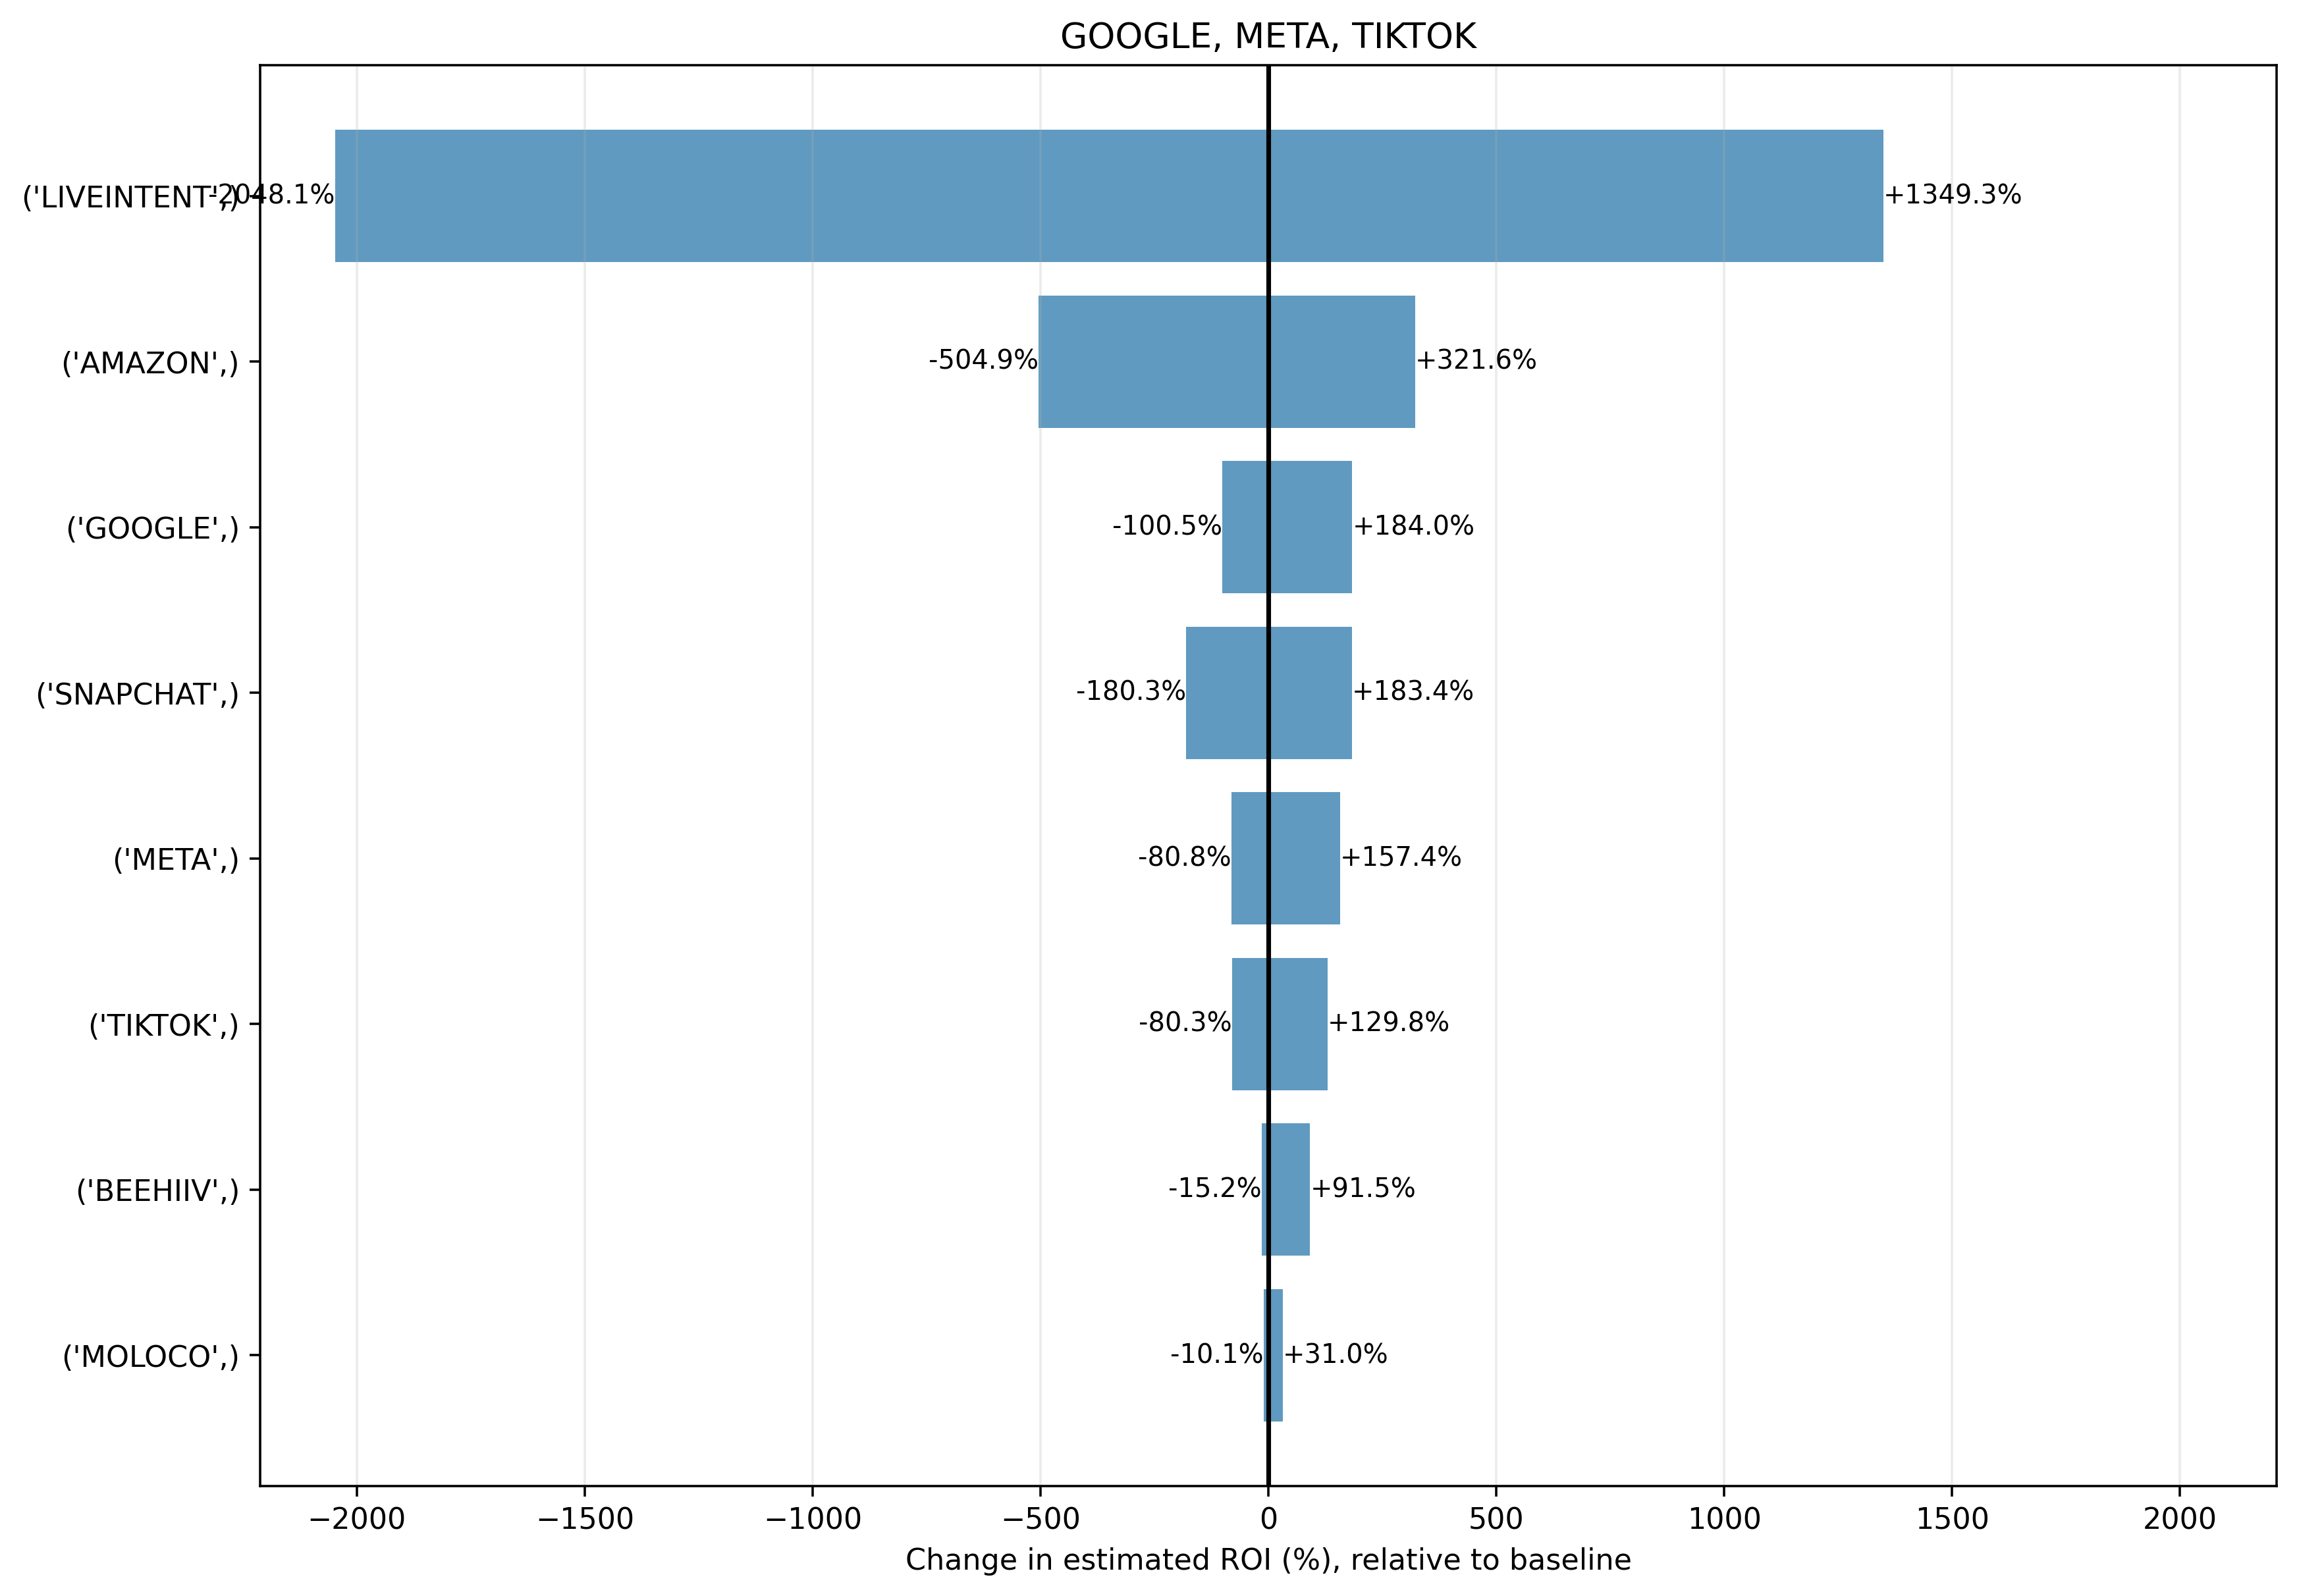
\includegraphics[width=0.93\textwidth]{img/BLUEALPHA1-fig1.png}
\caption{Fig. 1: ROI tornado summary for linked-target sensitivity (\texttt{google, meta, tiktok}).}
\label{fig:tornado_roi}
\end{figure}

\subsection*{Finding 2: Normal priors are less stable than LogNormal in this run set}
Across non-baseline tornado rows, the mean absolute ROI percent change is higher for Normal priors than for LogNormal priors (Normal: 248.41\%; LogNormal: 163.19\%). Figure~\ref{fig:heatmap} supports this pattern by showing high-response regions in the $\mu \times \sigma$ grid for the most sensitive entries.

\begin{figure}[H]
\centering
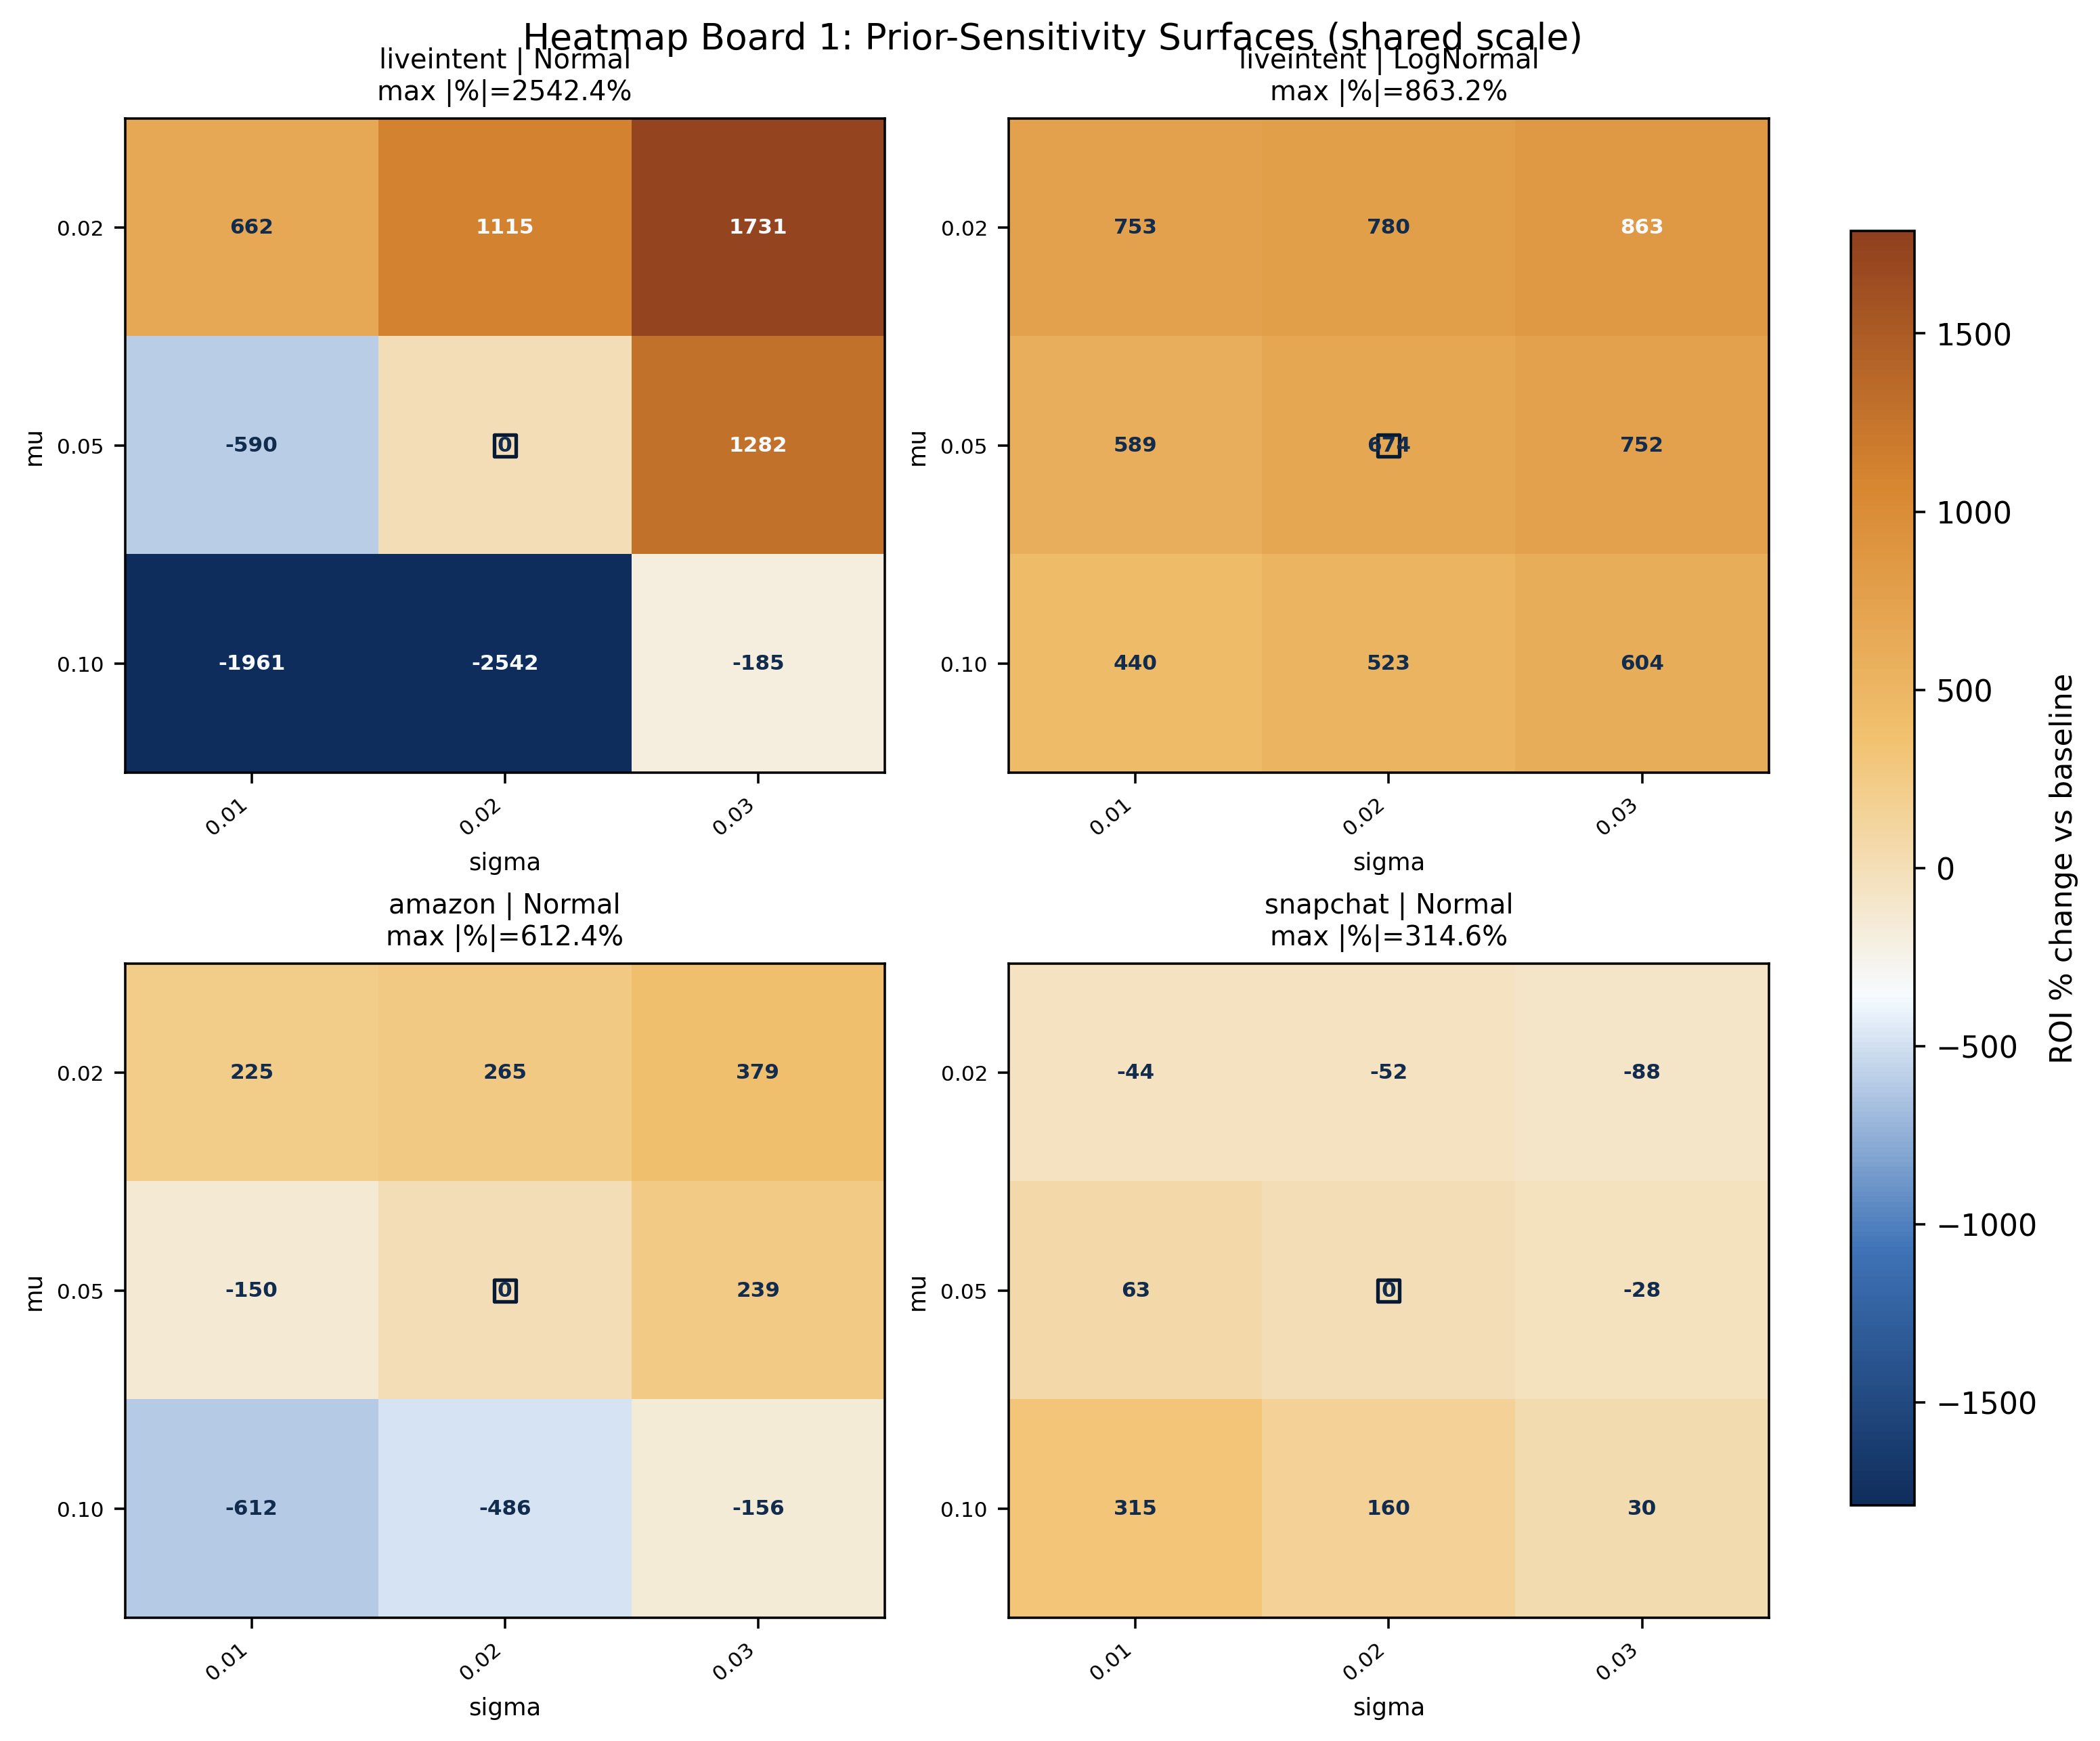
\includegraphics[width=0.93\textwidth]{img/BLUEALPHA1-fig2.png}
\caption{Fig. 2: Heatmap board (shared scale) for top sensitivity entries in the linked-target experiment.}
\label{fig:heatmap}
\end{figure}

\subsection*{Finding 3: Value-scaled sensitivity highlights business exposure}
Figure~\ref{fig:tornado_dollar} translates sensitivity into dollar units. The largest maximum absolute value deltas are concentrated in google and snapchat, then liveintent and tiktok. This indicates that channels with moderate percent instability can still represent high business exposure when spend volume is large.

\begin{figure}[H]
\centering
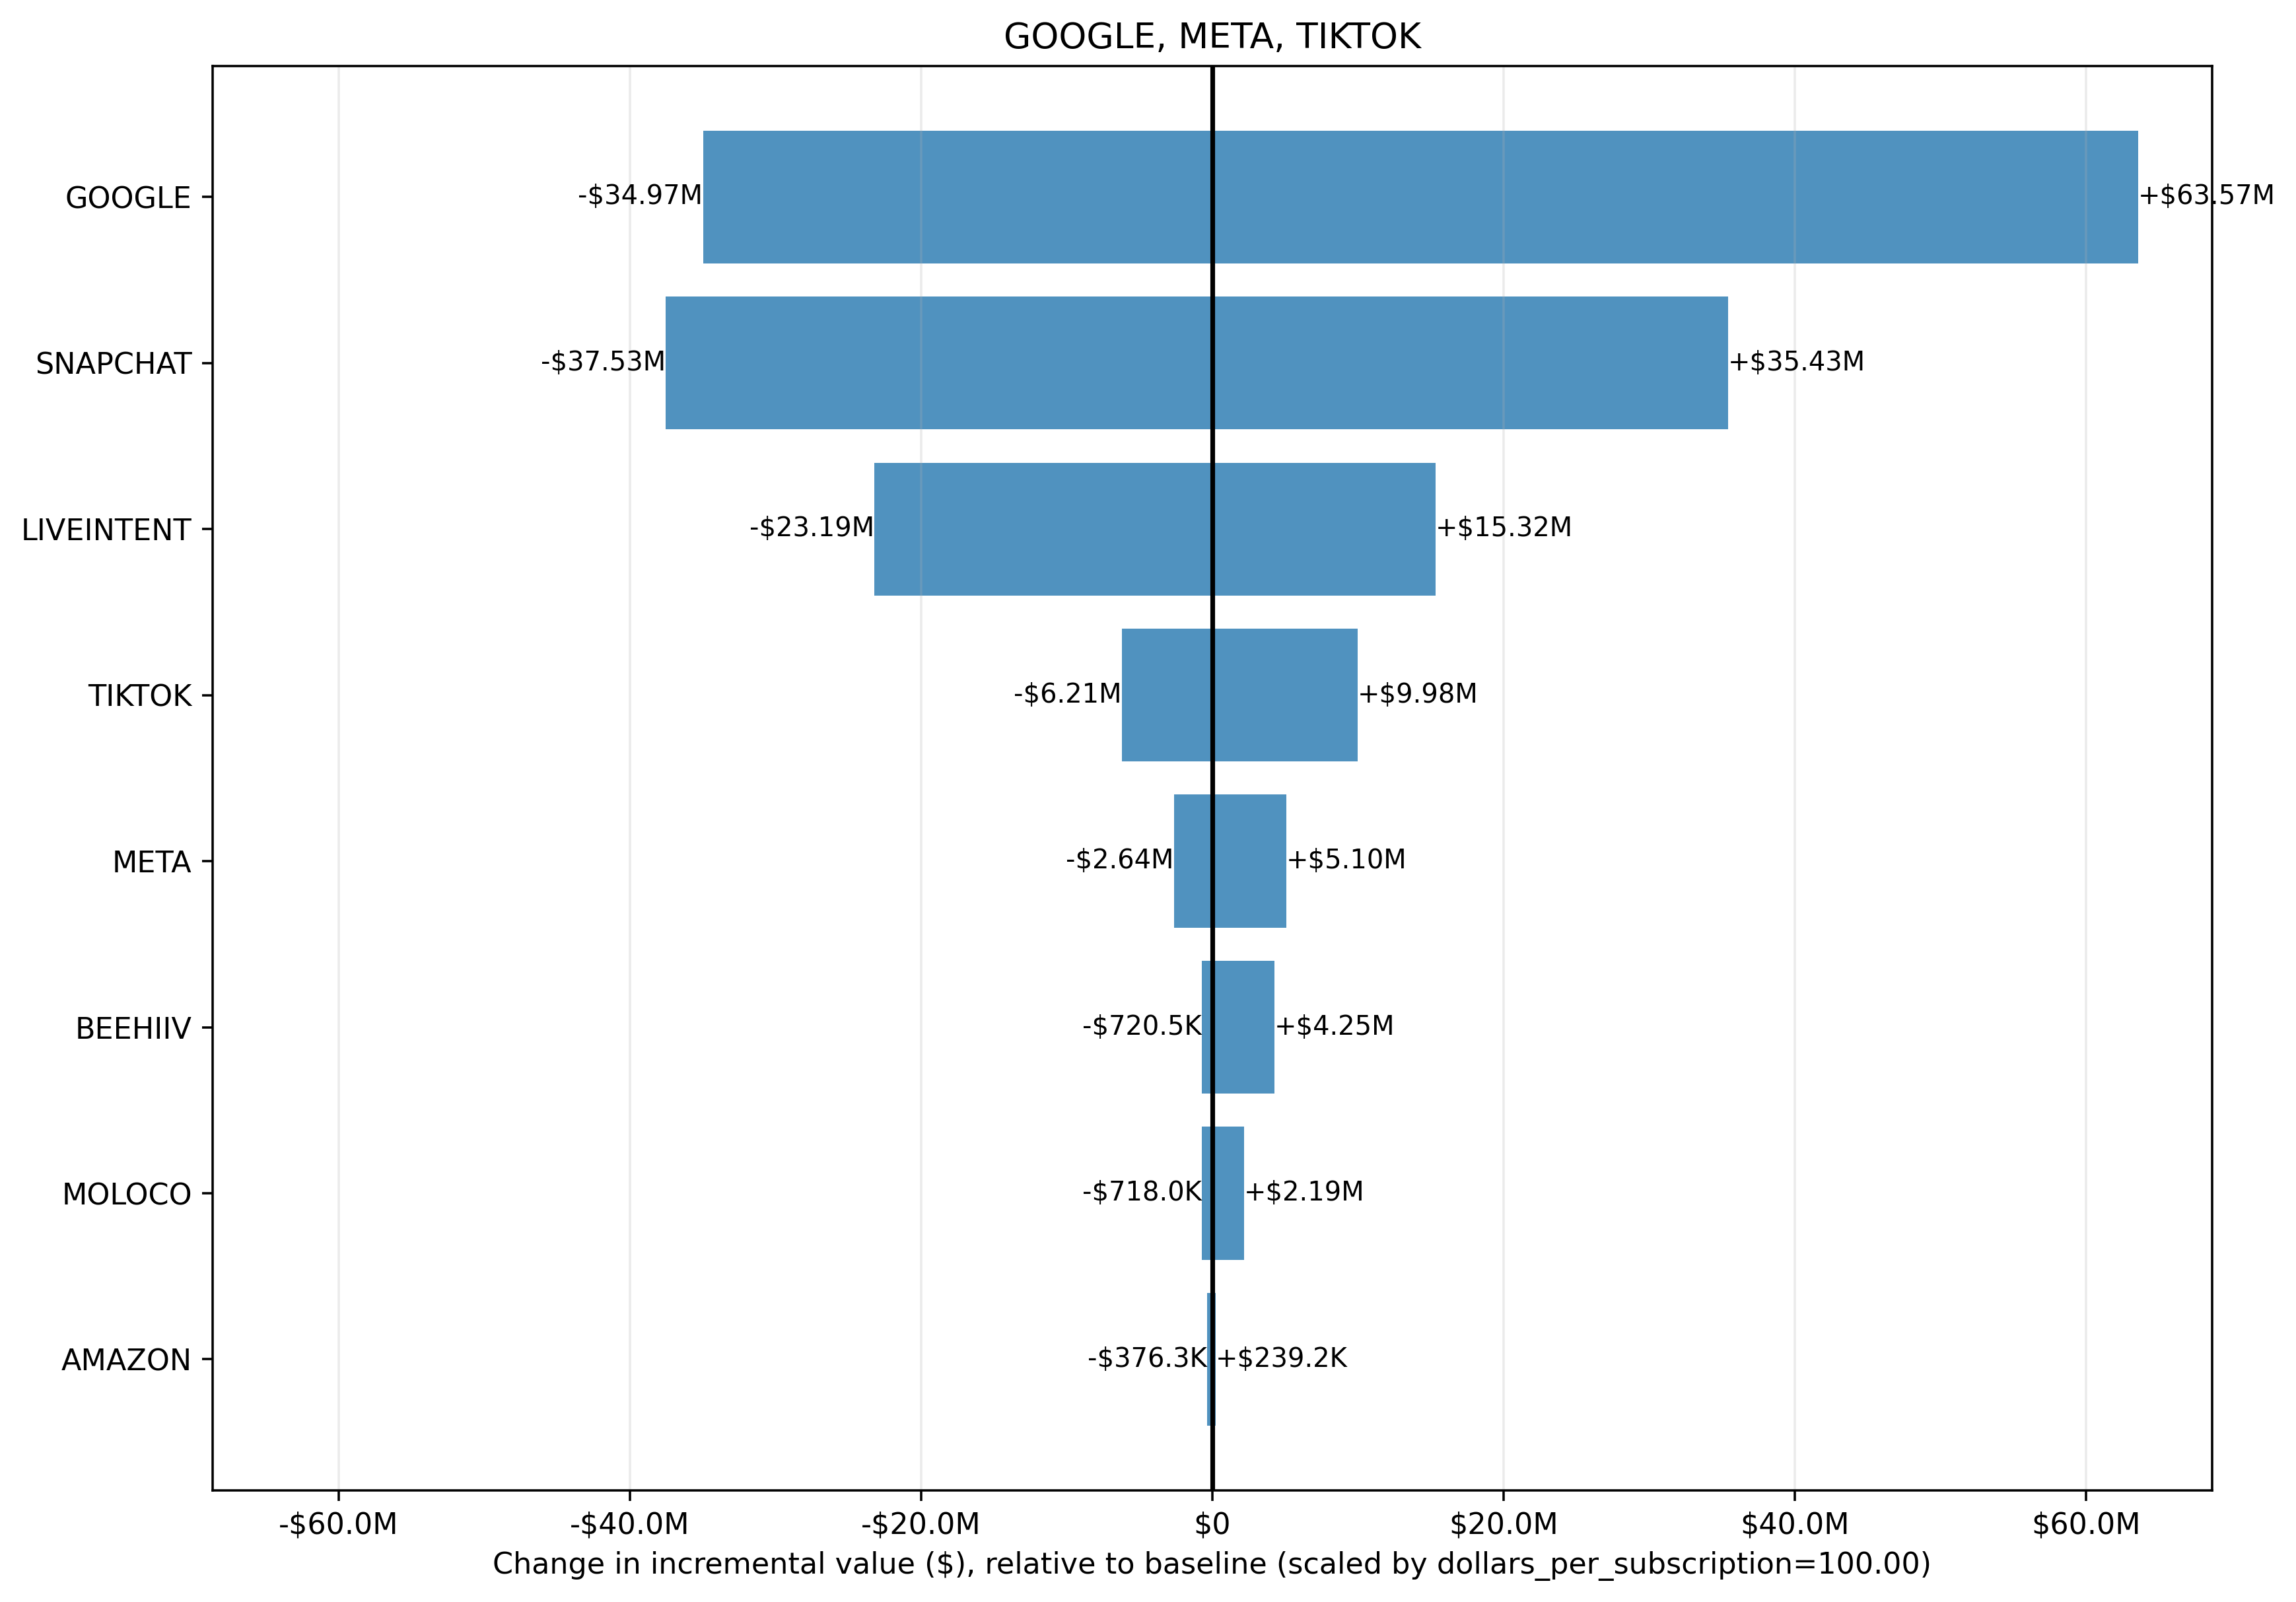
\includegraphics[width=0.93\textwidth]{img/BLUEALPHA1-fig3.png}
\caption{Fig. 3: Dollar tornado summary (value-scaled impact relative to baseline).}
\label{fig:tornado_dollar}
\end{figure}

\subsection*{Finding 4: Diagnostics show meaningful model-quality variation}
Run-level diagnostics indicate that instability is not only a prior-magnitude issue; model quality checks also vary across grid points.

\begin{table}[H]
\centering
\caption{Run-level QC status summary (18 total runs)}
\label{tab:qc_status}
\begin{tabular}{|l|r|r|}
\hline
Status & Count & Percent of runs \\
\hline
PASS & 9 & 50.0\% \\
REVIEW & 2 & 11.1\% \\
FAIL & 7 & 38.9\% \\
\hline
\end{tabular}
\end{table}

Among non-pass runs, the most common primary checks were Convergence and Baseline. This reinforces the need to combine sensitivity ranking with QC filtering before recommending priors.

\section{Discussion}
Overall, Winter-quarter results show that the framework is operational and informative: we can run linked-target experiments, aggregate ROI and value impacts, and produce diagnostics-rich summaries. The strongest practical insight is that sensitivity and business impact should be interpreted jointly. Large percent swings can appear when baseline ROI is small, while large spend channels can show substantial dollar exposure even when percent swings are not the highest.

The current results also surface two methodological cautions. First, sensitivity conclusions are conditional on the tested prior grid; they are not a global guarantee of robustness. Second, run failures and convergence flags can confound interpretation if not screened. For this reason, our recommendation logic prioritizes non-fail scenarios and keeps QC status visible in downstream summaries.

\section{Future Work}
Spring-quarter work will focus on four concrete extensions.

\begin{enumerate}
  \item \textbf{Failure analysis and grid refinement.} Use QC failure modes (especially convergence and baseline checks) to tighten or shift prior grids for unstable regions.
  \item \textbf{Richer perturbation scope.} Extend sensitivity beyond ROI prior hyperparameters to structural MMM components (for example, adstock and saturation assumptions).
  \item \textbf{Validation and calibration.} Compare high-sensitivity channels against external evidence (experiments, benchmarks, or historical constraints) to calibrate priors.
  \item \textbf{Cross-scenario generalization.} Replicate linked-target runs across additional target sets and datasets to test whether observed sensitivity patterns persist.
\end{enumerate}

\begin{thebibliography}{9}
\bibitem{meridian_model_spec}
Google for Developers.
\newblock \emph{Model specification | Meridian}.
\newblock \url{https://developers.google.com/meridian/docs/advanced-modeling/model-spec}.
\newblock Accessed March 20, 2026.

\bibitem{meridian_configure}
Google for Developers.
\newblock \emph{Configure the model | Meridian}.
\newblock \url{https://developers.google.com/meridian/docs/user-guide/configure-model}.
\newblock Accessed March 20, 2026.

\bibitem{jin2017}
Yuxue Jin, Yueqing Wang, Yunting Sun, David Chan, and Jim Koehler.
\newblock \emph{Bayesian Methods for Media Mix Modeling with Carryover and Shape Effects}.
\newblock Google Research publication, 2017.
\newblock \url{https://research.google/pubs/bayesian-methods-for-media-mix-modeling-with-carryover-and-shape-effects/}.
\end{thebibliography}

\section*{Appendix: Reproducibility Notes}
Main report source: \texttt{docs/reports/interim/BLUEALPHA1-interim-report-w26.tex}

Figure copies for submission:
\begin{itemize}
  \item \texttt{docs/reports/interim/img/BLUEALPHA1-fig1.png}
  \item \texttt{docs/reports/interim/img/BLUEALPHA1-fig2.png}
  \item \texttt{docs/reports/interim/img/BLUEALPHA1-fig3.png}
  \item \texttt{docs/reports/interim/img/BLUEALPHA1-fig4.png}
\end{itemize}

All copied figures were regenerated from the current repo outputs at approximately 320 dpi.

\end{document}
